\documentclass{beamer}
\input{../utils/preamble}
\createdgmtitle{5}
%--------------------------------------------------------------------------------
\begin{document}
%--------------------------------------------------------------------------------
\begin{frame}[noframenumbering,plain]
	\titlepage
	\resetonslide
\end{frame}
%=======
\begin{frame}{Recap of Previous Lecture}
	\myfootnotewithlink{https://arxiv.org/abs/1711.00937}{Oord A., Vinyals O., Kavukcuoglu K. Neural Discrete Representation Learning, 2017} 
	\vspace{-0.3cm}
	\begin{block}{Assumptions}
		\begin{itemize}
			\item Let $c \sim \Cat(\bpi)$, where 
			\vspace{-0.6cm}
			\[
				\bpi = (\pi_1, \dots, \pi_K), \quad \pi_k = P(c = k), \quad \sum_{k=1}^K \pi_k = 1.
			\]
			\vspace{-0.7cm}
			\item Suppose the VAE includes a discrete latent variable $c$ with prior $p(c) = \text{Uniform}\{1, \dots, K\}$.
		\end{itemize}
	\end{block}
	\vspace{-0.3cm}
	\begin{block}{ELBO}
		\vspace{-0.6cm}
		\[
			\cL_{\bphi, \btheta}(\bx)  = \bbE_{q_{\bphi}(c| \bx)} \log \pt(\bx| c) - {\color{olive} \KL(q_{\bphi}(c| \bx) \| p(c))} \rightarrow \max_{\bphi, \btheta}.
		\]
	\end{block}
	\vspace{-1.0cm}
	\[
		\KL(q_{\bphi}(c| \bx) \| p(c)) = - \Ent(q_{\bphi}(c| \bx)) + \log K. 
	\]		
	\vspace{-0.5cm}
	\begin{itemize}
		\item Our encoder must output the discrete distribution $q_{\bphi}(c| \bx)$.
		\item We'll require an analogue of the reparameterization trick for discrete $q_{\bphi}(c| \bx)$.
		\item Our decoder $\pt(\bx| c)$ has input the discrete variable $c$.
	\end{itemize}
\end{frame}
%=======

\begin{frame}{Recap of Previous Lecture}
	\myfootnotewithlink{https://arxiv.org/abs/1711.00937}{Oord A., Vinyals O., Kavukcuoglu K. Neural Discrete Representation Learning, 2017} 
	\begin{block}{Assumptions}
		\begin{itemize}
			\item Let $c \sim \Cat(\bpi)$, where 
			\vspace{-0.6cm}
			\[
				\bpi = (\pi_1, \dots, \pi_K), \quad \pi_k = P(c = k), \quad \sum_{k=1}^K \pi_k = 1.
			\]
			\vspace{-0.7cm}
			\item Suppose the VAE employs a discrete latent code $c$, with prior $p(c) = \text{Uniform}\{1, \dots, K\}$.
		\end{itemize}
	\end{block}
	\vspace{-0.3cm}
	\begin{block}{ELBO}
		\vspace{-0.7cm}
		\[
			\cL_{\bphi, \btheta}(\bx)  = \bbE_{q_{\bphi}(c| \bx)} \log \pt(\bx| c) - {\color{olive} \KL(q_{\bphi}(c| \bx) \,\|\, p(c))} \rightarrow \max_{\bphi, \btheta}.
		\]
	\end{block}
	\vspace{-1.0cm}
	\[
		\KL(q_{\bphi}(c| \bx) \,\|\, p(c)) = - \Ent(q_{\bphi}(c| \bx)) + \log K. 
	\]		
	\vspace{-0.5cm}
	\begin{block}{Vector Quantization}
		Define the codebook $\{\be_k\}_{k=1}^K$, where $\be_k \in \bbR^L$ and $K$ is the size of the dictionary.
		\vspace{-0.3cm}
		\[
			\bz_q = \bq (\bz) = \be_{k^*}, \quad \text{where}\;\; k^* = \argmin_k \| \bz - \be_k \|.
		\] 
		\vspace{-0.7cm}
	\end{block}
\end{frame}
%=======
\begin{frame}{Recap of Previous Lecture}
	\myfootnotewithlink{https://arxiv.org/abs/1711.00937}{Oord A., Vinyals O., Kavukcuoglu K. Neural Discrete Representation Learning, 2017} 
	\begin{figure}
		\centering
		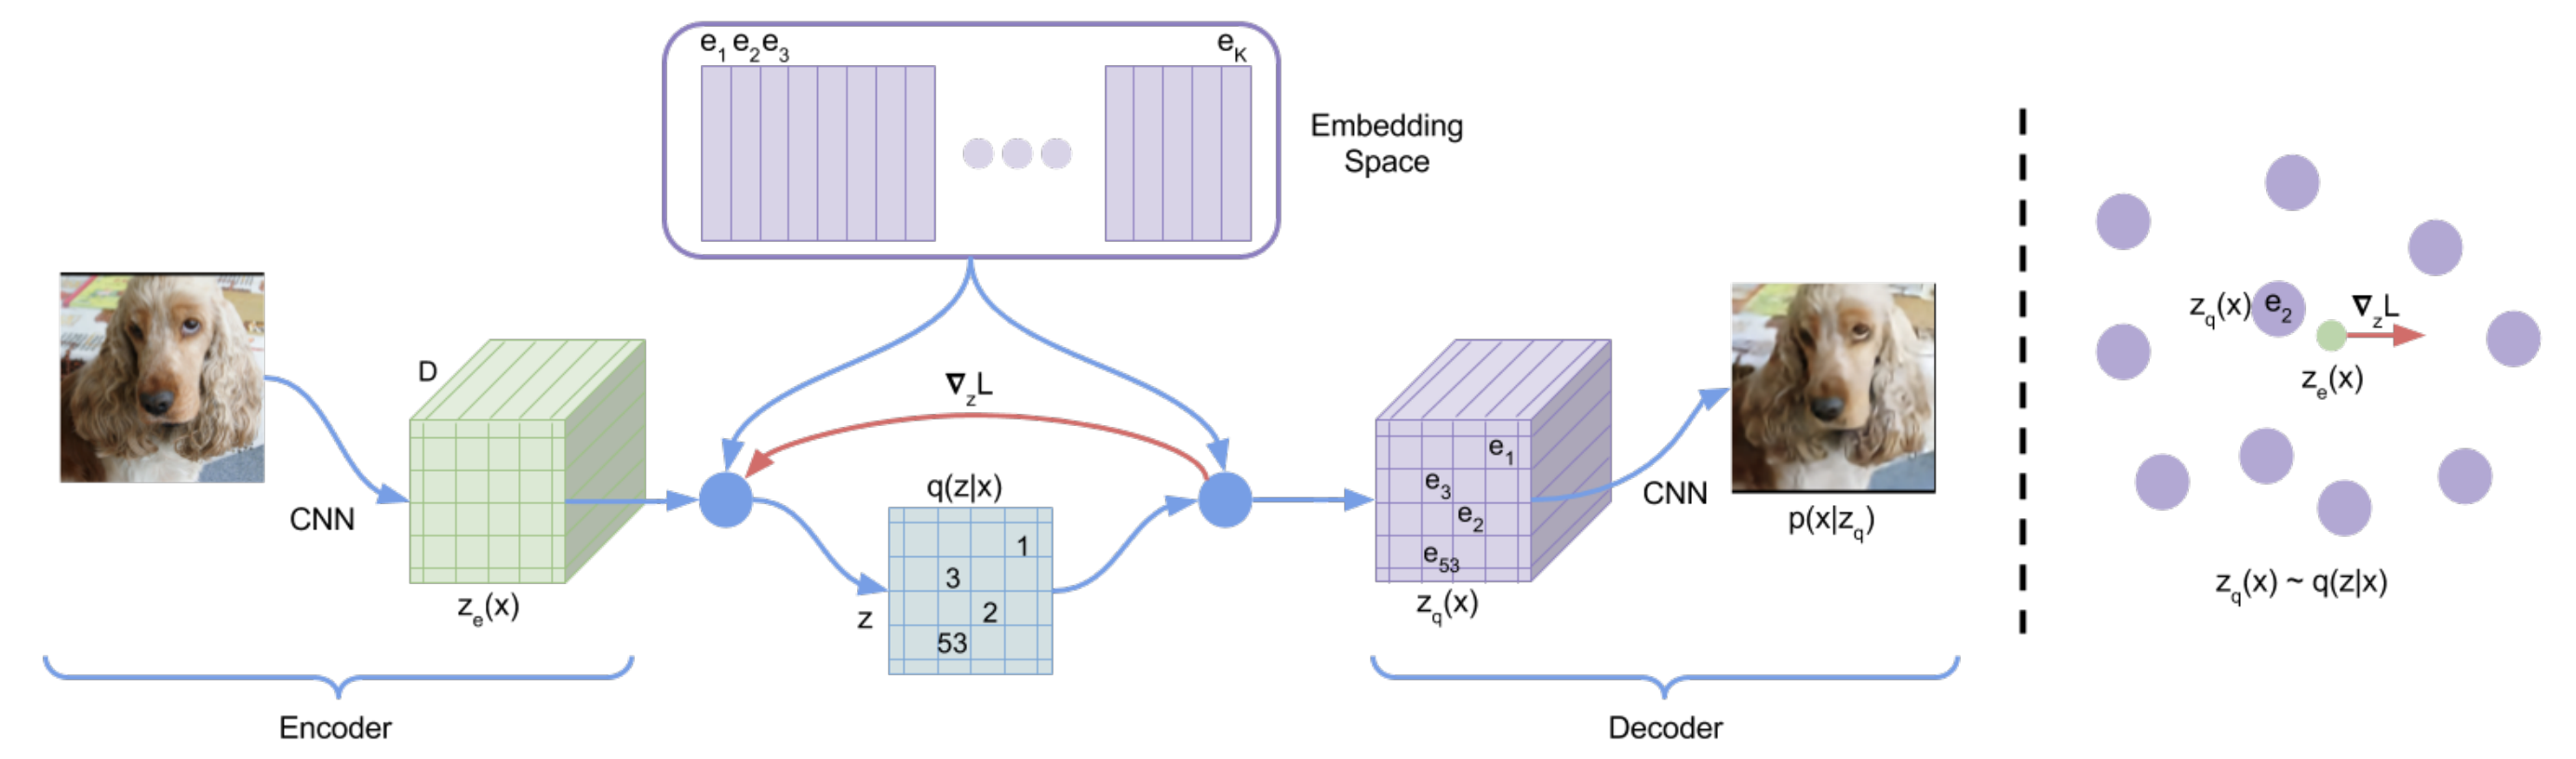
\includegraphics[width=0.85\linewidth]{figs/vqvae}
	\end{figure}
	\vspace{-0.3cm}
	\begin{block}{Deterministic Variational Posterior}
		\vspace{-0.3cm}
		\[
			q_{\bphi}(c_{ij} = k^* | \bx) = \begin{cases}
				1,  & \text{if}\;\; k^* = \argmin_k \| [\bz_e]_{ij} - \be_k \|; \\
				0,  & \text{otherwise}.
			\end{cases}
		\]
		\vspace{-0.5cm}
	\end{block}
	\begin{block}{ELBO}
		\vspace{-0.6cm}
		\[
			\cL_{\bphi, \btheta}(\bx)  = \bbE_{q_{\bphi}(c| \bx)} \log \pt(\bx| \be_{c}) - \log K =  \log \pt(\bx| \bz_q) - \log K.
		\]
		\vspace{-0.6cm}
	\end{block}
	\begin{block}{Straight-Through Gradient Estimation}
		\vspace{-0.6cm}
		\[
			\frac{\partial \log p(\bx | \bz_q , \btheta)}{\partial \bphi} = \frac{\partial \log \pt(\bx| \bz_q)}{\partial \bz_q} \cdot {\color{red}\frac{\partial \bz_q}{\partial \bphi}} \approx \frac{\partial \log \pt(\bx| \bz_q)}{\partial \bz_q} \cdot \frac{\partial \bz_e}{\partial \bphi}
		\]
	\end{block}
\end{frame}
%=======
\begin{frame}{Recap of Previous Lecture}
	\myfootnotewithlink{http://approximateinference.org/accepted/HoffmanJohnson2016.pdf}{Hoffman M. D., Johnson M. J. ELBO surgery: yet another way to carve up the variational evidence lower bound, 2016}
	\vspace{-0.3cm}
	\begin{block}{Theorem}
		\vspace{-0.6cm}
		\[
			\frac{1}{n} \sum_{i=1}^n \KL(q_{\bphi}(\bz| \bx_i) \,\|\, p(\bz)) = \KL({\color{teal}q_{\text{agg}, \bphi}(\bz) } \,\|\, p(\bz)) + \bbI_{q} [\bx, \bz].
		\]
		\vspace{-0.6cm}
	\end{block}
	\begin{block}{ELBO Surgery}
		\vspace{-0.5cm}
		{\small
		\[		  
		    \frac{1}{n} \sum_{i=1}^n \cL_{\bphi, \btheta}(\bx_i) = \underbrace{\frac{1}{n} \sum_{i=1}^n \bbE_{q_{\bphi}(\bz| \bx_i)} \log \pt(\bx_i | \bz)}_{\text{Reconstruction Loss}}
		    - \underbrace{\vphantom{\sum_{i=1}^n} \bbI_q [\bx, \bz]}_{\text{MI}} - \underbrace{\vphantom{\sum_{i=1}^n} \KL({\color{teal}q_{\text{agg}, \bphi}(\bz)} \,\|\, {\color{violet}p(\bz)})}_{\text{Marginal KL}}
		\]}
	\end{block}
	\vspace{-0.7cm}
	\begin{block}{Optimal Prior}
		\vspace{-0.7cm}
		\[
			\KL(q_{\text{agg}, \bphi}(\bz) \,\|\, p(\bz)) = 0 \ \Leftrightarrow \ p (\bz) = q_{\text{agg}}(\bz) = \frac{1}{n} \sum_{i=1}^n q_{\bphi}(\bz| \bx_i).
		\]
		\vspace{-0.5cm}\\
		Thus, the optimal prior distribution $p(\bz)$ is the aggregated variational posterior $q_{\text{agg}, \bphi}(\bz)$.
	\end{block}
\end{frame}
%=======
\begin{frame}{Recap of Previous Lecture}
	\myfootnotewithlink{https://arxiv.org/abs/1611.02731}{Chen X. et al. Variational Lossy Autoencoder, 2016}
	\begin{itemize}
		\item Standard Gaussian $p(\bz) = \cN(0, \bI)$ $\Rightarrow$ over-regularization.
		\item $p(\bz) = q_{\text{agg}, \bphi}(\bz) = \frac{1}{n}\sum_{i=1}^n q_{\bphi}(\bz| \bx_i)$ $\Rightarrow$ overfitting and extremely high computational cost.
	\end{itemize}
	\begin{block}{Revisiting ELBO}
		\vspace{-0.4cm}
		\[
		\frac{1}{n}\sum_{i=1}^n \cL_{\bphi, \btheta}(\bx_i) = \text{RL} - \text{MI} -  \KL(q_{\text{agg}, \bphi}(\bz) \,\|\, {\color{violet}p_{\blambda}(\bz)})
		\]
		This is the forward KL divergence with respect to $p_{\blambda}(\bz)$.
	\end{block}
	\begin{block}{ELBO with Learnable VAE Prior}
		\vspace{-0.6cm}
		{\small
			\begin{multline*}
				\cL_{\bphi, \btheta}(\bx) = \bbE_{q_{\bphi}(\bz| \bx)} \left[ \log \pt(\bx | \bz) + {\color{violet}\log p_{\blambda}(\bz)} - \log q_{\bphi}(\bz| \bx) \right] \\
				= \bbE_{q_{\bphi}(\bz| \bx)} \Bigl[ \log \pt(\bx | \bz) + \underbrace{ \Bigl({\color{violet} \log p(f_{\blambda}(\bz)) + \log \left| \det (\bJ_\bff) \right|} \Bigr) }_{\text{flow-based prior}} - \log q_{\bphi}(\bz| \bx) \Bigr] 
			\end{multline*}
		}
		\vspace{-0.5cm}
		\[
			\bz = \bff^{-1}_{\blambda}(\bz^*) = \bg_{\blambda}(\bz^*), \quad \bz^* \sim p(\bz^*) = \cN(0, \bI)
		\]
	\end{block}
	\vspace{-0.5cm}
\end{frame}
%=======
\begin{frame}{Outline}
	\tableofcontents
\end{frame}
%=======
\begin{frame}{Outline}
	\tableofcontents
\end{frame}
%=======
\section{Likelihood-Free Learning}
%=======
\begin{frame}{Likelihood-Based Models}
	\myfootnotewithlink{https://arxiv.org/abs/1511.01844}{Theis L., Oord A., Bethge M. A Note on the Evaluation of Generative Models, 2015}
	\begin{minipage}[t]{0.48\columnwidth}
		\vspace{-0.3cm}
		\begin{block}{Poor Likelihood \\ High-Quality Samples}
			\vspace{-0.3cm}
			\[
				p_1(\bx) = \frac{1}{n} \sum_{i=1}^n \cN(\bx | \bx_i, \epsilon \bI)
			\]
			If $\epsilon$ is very small, this model produces excellent, sharp samples but achieves poor likelihoods on test data.
		\end{block}	
	\end{minipage}%
	\begin{minipage}[t]{0.52\columnwidth}
		\eqpause
		\vspace{-0.3cm}
		\begin{block}{High Likelihood \\ Poor Samples}
			\vspace{-0.5cm}
			\[
				p_2(\bx) = 0.01p(\bx) + 0.99p_{\text{noise}}(\bx)
			\]
			\vspace{-1.0cm}
			\begin{multline*}
				\log \left[ 0.01p(\bx) + 0.99p_{\text{noise}}(\bx) \right] \geq \\ \geq \log \left[ 0.01p(\bx) \right]  = \log p(\bx) - \log 100
			\end{multline*}
			This model contains mostly noisy, irrelevant samples; for high dimensions, $\log p(\bx)$ scales linearly with $m$.
		\end{block}
	\end{minipage}
	\eqpause
	\begin{itemize}
		\item Likelihood isn't always a suitable metric for evaluating generative models.
		\item Sometimes, the likelihood function can't even be computed exactly.
	\end{itemize}
\end{frame}
%=======
\begin{frame}{Likelihood-Free Learning}
	\begin{block}{Motivation}
	 We're interested in approximating the true data distribution~$\pd(\bx)$.
	Instead of searching over all distributions, let's learn a model $\pt(\bx) \approx \pd(\bx)$.
	\end{block}
	\eqpause
	Suppose we have two sets of samples: 
	\begin{itemize}
		\item $\{\bx_i\}_{i=1}^{n_1} \sim \pd(\bx)$ — real data;
		\item $\{\bx_i\}_{i=1}^{n_2} \sim \pt(\bx)$ — generated (fake) data.
	\end{itemize}
	\eqpause
	Define a discriminative model (classifier):
	\[
		p(y = 1 | \bx) = P(\bx \sim \pd(\bx)); \quad p(y = 0 | \bx) = P(\bx \sim \pt(\bx))
	\]
	\eqpause
	\vspace{-0.5cm}
	\begin{block}{Assumption}
		The generative model $\pt(\bx)$ matches $\pd(\bx)$ if a discriminative model $p(y | \bx)$ can't distinguish between them --- that is, if $p(y = 1 | \bx) = 0.5$ for every $\bx$.
	\end{block}
\end{frame}
%=======
\begin{frame}{Generative Adversarial Networks (GAN)}
	\myfootnotewithlink{https://arxiv.org/abs/1406.2661}{Goodfellow I. J. et al. Generative Adversarial Networks, 2014}
	\begin{itemize}
		\item The more expressive the discriminator, the closer we get to the optimal $\pt(\bx)$.
		\item Standard classifiers are trained by minimizing cross-entropy loss $-\bbE_{\hat{p}(\bx, y)} \log p(y | \bx)$ with $\hat{p}(\bx, y) = \frac{1}{2} [y=1]\pd(\bx) + \frac{1}{2} [y=0]\pt(\bx)$.
	\end{itemize}
	\eqpause
	\begin{block}{Cross-Entropy for Discriminator}
		\vspace{-0.3cm}
		\[
			\min_{p(y | \bx)} \left[ - \bbE_{\pd(\bx)} \log p(y = 1 | \bx) - \bbE_{\pt(\bx)} \log p(y = 0 | \bx) \right] 
		\]
		\[
			\max_{p(y | \bx)} \left[\bbE_{\pd(\bx)} \log p(y = 1 | \bx) + \bbE_{\pt(\bx)} \log p(y = 0 | \bx) \right] 
		\]
	\end{block}
	\eqpause
	\vspace{-0.3cm}
	\begin{block}{Generative Model}
		Suppose $\pt(\bx, \bz) = \pt(\bx| \bz) p(\bz)$, where $p(\bz)$ is a base distribution, and $\pt(\bx | \bz) = \delta (\bx - \bG_{\btheta}(\bz))$ is deterministic.
	\end{block}
\end{frame}
%=======
\begin{frame}{Generative Adversarial Networks (GAN)}
	\myfootnotewithlink{https://arxiv.org/abs/1406.2661}{Goodfellow I. J. et al. Generative Adversarial Networks, 2014}
	\begin{block}{Cross-Entropy for Discriminative Model}
		\vspace{-0.3cm}
		\[
			\max_{p(y | \bx)} \left[\bbE_{\pd(\bx)} \log p(y = 1 | \bx) + \bbE_{\pt(\bx)} \log p(y = 0 | \bx) \right] 
		\]
	\end{block}
	\eqpause
	\begin{itemize}
		\item \textbf{Discriminator:} A classifier $p_{\bphi}(y = 1 | \bx) = D_{\bphi}(\bx) \in [0, 1]$, distinguishing real and generated samples. The discriminator aims to \textbf{maximize} cross-entropy.
		\item \textbf{Generator:} The generative model $\bx = \bG_{\btheta}(\bz),\; \bz \sim p(\bz)$, seeks to fool the discriminator. The generator aims to \textbf{minimize} cross-entropy.
	\end{itemize}
	\eqpause
	\begin{block}{GAN Objective}
		\vspace{-0.5cm}
		\[
			\min_{G} \max_D \left[ \bbE_{\pd(\bx)} \log D(\bx) + \bbE_{\pt(\bx)} \log (1 - D(\bx)) \right] 
		\]
		\eqpause
		\[
			\min_{G} \max_D \left[ \bbE_{\pd(\bx)} \log D(\bx) + \bbE_{p(\bz)} \log (1 - D(\bG(\bz))) \right]
		\]
	\end{block}
\end{frame}
%=======
\section{Generative Adversarial Networks (GAN)}
%=======
\begin{frame}{Generative Models Zoo}
	\begin{tikzpicture}[
	 	basic/.style  = {draw, text width=2cm, drop shadow, rectangle},
	 	root/.style   = {basic, rounded corners=2pt, thin, text height=1.1em, text width=7em, align=center, fill=blue!40},
	 	level 1/.style={sibling distance=55mm},
	 	level 2/.style = {basic, rounded corners=6pt, thin, align=center, fill=blue!20, text height=1.1em, text width=9em, sibling distance=38mm},
	 	level 3/.style = {basic, rounded corners=6pt, thin,align=center, fill=blue!20, text width=8.5em},
	 	level 4/.style = {basic, thin, align=left, fill=pink!30, text width=7em},
	 	level 5/.style = {basic, thin, align=left, fill=pink!90, text width=7em},
		edge from parent/.style={->,draw},
		>=latex]
		
		\node[root] {\Large Generative Models}
		child {node[level 2] (c1) {Likelihood-Based}
			child {node[level 3] (c11) {Tractable Density}}
			child {node[level 3] (c12) {Approximate Density}}
		}
		child {node[level 2] (c2) {Likelihood-Free}};
		
		\begin{scope}[every node/.style={level 4}]
		\node [below of = c11, yshift=-5pt, xshift=10pt] (c111) {Autoregressive Models};
		\node [below of = c111, yshift=-5pt] (c112) {Normalizing Flows};
		
		\node [below of = c12, xshift=10pt] (c121) {VAEs};
		\node [below of = c121] (c122) {Diffusion Models};
		\end{scope}
		
		\begin{scope}[every node/.style={level 5}]
		\node [below of = c2, xshift=10pt] (c21) {GANs};
		\end{scope}
		
		\foreach \value in {1,2}
		\draw[->] (c11.194) |- (c11\value.west);
		
		\foreach \value in {1,2}
		\draw[->] (c12.194) |- (c12\value.west);
		
		\draw[->] (c2.194) |- (c21.west);
		
	\end{tikzpicture}
\end{frame}
%=======
\begin{frame}{GAN Optimality}
	\myfootnotewithlink{https://arxiv.org/abs/1406.2661}{Goodfellow I. J. et al. Generative Adversarial Networks, 2014}
	\begin{block}{Theorem}
		The minimax game
		\vspace{-0.3cm}
		\[
			\min_{G} \max_D \Bigl[ \underbrace{\bbE_{\pd(\bx)} \log D(\bx) + \bbE_{p(\bz)} \log (1 - D(\bG(\bz)))}_{V(G, D)} \Bigr]
		\]
		\vspace{-0.5cm} \\
		achieves its global optimum when $\pd(\bx) = \pt(\bx)$, and $D^*(\bx) = 0.5$.
	\end{block}
	\eqpause
	\begin{block}{Proof (Fixed $G$)}
		\vspace{-0.5cm}
		\begin{align*}
			V(G, D) &= \bbE_{\pd(\bx)} \log D(\bx) + \bbE_{\pt(\bx)} \log (1 - D(\bx)) \\
			\nextonslide{&= \int \underbrace{\left[ \pd(\bx) \log D(\bx) + \pt(\bx)\log (1 - D(\bx)) \right]}_{y(D)} d \bx}
		\end{align*}
		\eqpause
		\vspace{-0.2cm}
		\[
			\frac{d y(D)}{d D} = \frac{\pd(\bx)}{D(\bx)} - \frac{\pt(\bx)}{1 - D(\bx)} = 0 \qquad \Rightarrow \quad D^*(\bx) = \frac{\pd(\bx)}{\pd(\bx) + \pt(\bx)}
		\]
	\end{block}
\end{frame}
%=======
\begin{frame}{GAN Optimality}
	\myfootnotewithlink{https://arxiv.org/abs/1406.2661}{Goodfellow I. J. et al. Generative Adversarial Networks, 2014}
	\begin{block}{Proof Continued (Fixed $D = D^*$)}
		\vspace{-0.5cm}
		{\small
		\begin{multline*}
			V(G, D^*) = \bbE_{\pd(\bx)} \log \left( \frac{\pd(\bx)}{\pd(\bx) + \pt(\bx)} \right) + \bbE_{\pt(\bx)} \log \left( \frac{\pt(\bx)}{\pd(\bx) + \pt(\bx)}\right)  \\
		 \nextonslide{= \KL \left(\pd(\bx) \,\|\, \frac{\pd(\bx) + \pt(\bx)}{2}\right) + \KL \left(\pt(\bx) \,\|\, \frac{\pd(\bx) + \pt(\bx)}{2}\right) - 2\log 2 \\}
		 \nextonslide{= 2\,\JSD(\pd(\bx) \,\|\, \pt(\bx)) - 2\log 2.}
		\end{multline*}
		}
	\end{block}
	\eqpause
	\vspace{-0.3cm}
	\begin{block}{Jensen-Shannon Divergence (Symmetric KL Divergence)}
		\vspace{-0.3cm}
		\[
			\JSD(\pd(\bx) \| \pt(\bx)) = \frac{1}{2} \left[\KL \left(\pd(\bx) \| {\color{teal}\star}\right) + \KL \left(\pt(\bx) \| {\color{teal}\star}\right) \right]
		\]
	\end{block}
	\eqpause
	This can be regarded as a proper distance metric!
	\[
		V(G^*, D^*) = -2\log 2, \quad \pd(\bx) = \pt(\bx), \quad  D^*(\bx) = 0.5.
	\]
\end{frame}
%=======
\begin{frame}{GAN Optimality}
	\myfootnotewithlink{https://arxiv.org/abs/1406.2661}{Goodfellow I. J. et al. Generative Adversarial Networks, 2014}
	\begin{block}{Theorem}
		The following minimax game 
		\vspace{-0.3cm}
		\[
		\min_{G} \max_D \Bigl[ \bbE_{\pd(\bx)} \log D(\bx) + \bbE_{p(\bz)} \log (1 - D(\bG(\bz))) \Bigr]
		\]
		\vspace{-0.5cm} \\
		achieves its global optimum precisely when $\pd(\bx) = \pt(\bx)$, and $D^*(\bx) = 0.5$.
	\end{block}
	\vspace{-0.2cm}
	\begin{block}{Expectations}
		If the generator can express \textbf{any} function and the discriminator is \textbf{optimal} at every step, the generator \textbf{will converge} to the target distribution.
	\end{block}
	\vspace{-0.3cm}
	\eqpause
	\begin{block}{Reality}
		\begin{itemize}
			\item Generator updates are performed in parameter space, and the discriminator is often imperfectly optimized.
			\item Generator and discriminator losses typically oscillate during GAN training.
		\end{itemize}
	\end{block}
\end{frame}
%=======
\begin{frame}{GAN Training}
	\myfootnotewithlink{https://arxiv.org/abs/1406.2661}{Goodfellow I. J. et al. Generative Adversarial Networks, 2014}

	Assume both generator and discriminator are parametric models: $D_{\bphi}(\bx)$ and $\bG_{\btheta}(\bz)$.
	\begin{block}{Objective}
		\vspace{-0.7cm}
		\[
		\min_{\btheta} \max_{\bphi} \left[ \bbE_{\pd(\bx)} \log D_{\bphi}(\bx) + \bbE_{p(\bz)} \log (1 - D_{\bphi}(\bG_{\btheta}(\bz))) \right]
		\]
		\vspace{-0.7cm}
	\end{block}
	\eqpause
	\begin{figure}
		\centering
		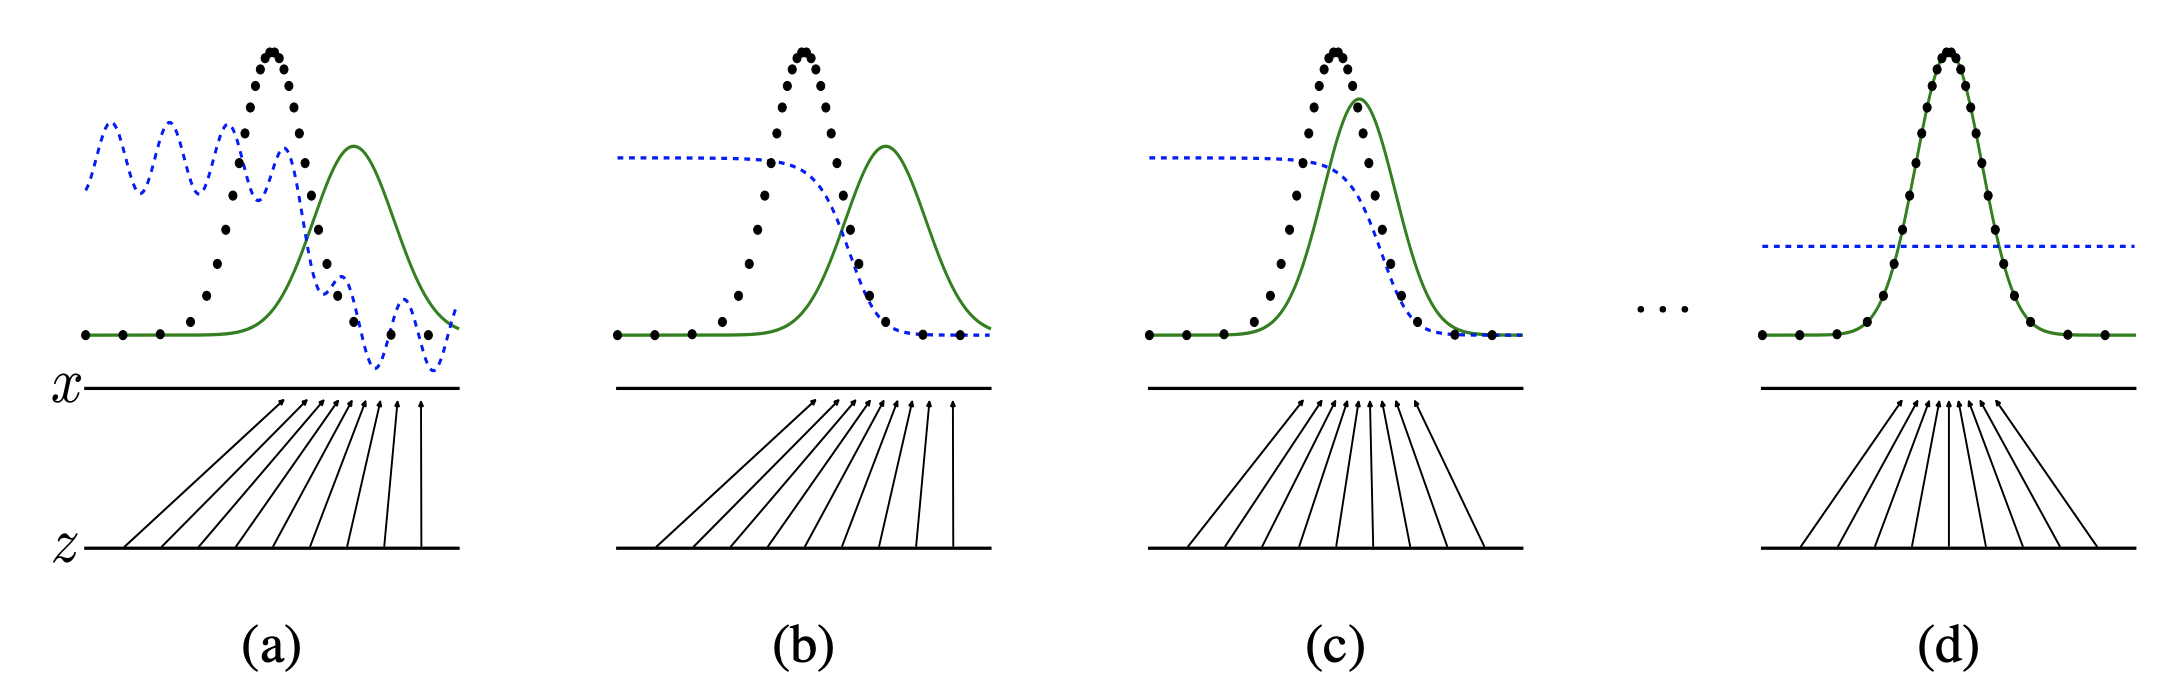
\includegraphics[width=1.0\linewidth]{figs/gan_1}
	\end{figure}
	\vspace{-0.5cm}
	\eqpause
	\begin{itemize}
		\item $\bz \sim p(\bz)$ is a latent variable.
		\item $\pt(\bx | \bz) = \delta(\bx - \bG_{\btheta}(\bz))$ serves as a deterministic decoder ({\color{gray}like normalizing flows}).
		\item There is no encoder present.
	\end{itemize}
\end{frame}
%=======
\begin{frame}{Mode Collapse}
	\myfootnote{\href{https://arxiv.org/abs/1406.2661}{Goodfellow I. J. et al. Generative Adversarial Networks, 2014} \\
		\href{https://arxiv.org/abs/1611.02163}{Metz L. et al. Unrolled Generative Adversarial Networks, 2016}}
	Mode collapse refers to the phenomenon where the generator in a GAN produces only one or a few different modes of the distribution.
	\vspace{-0.1cm}
	\begin{figure}
		\centering
		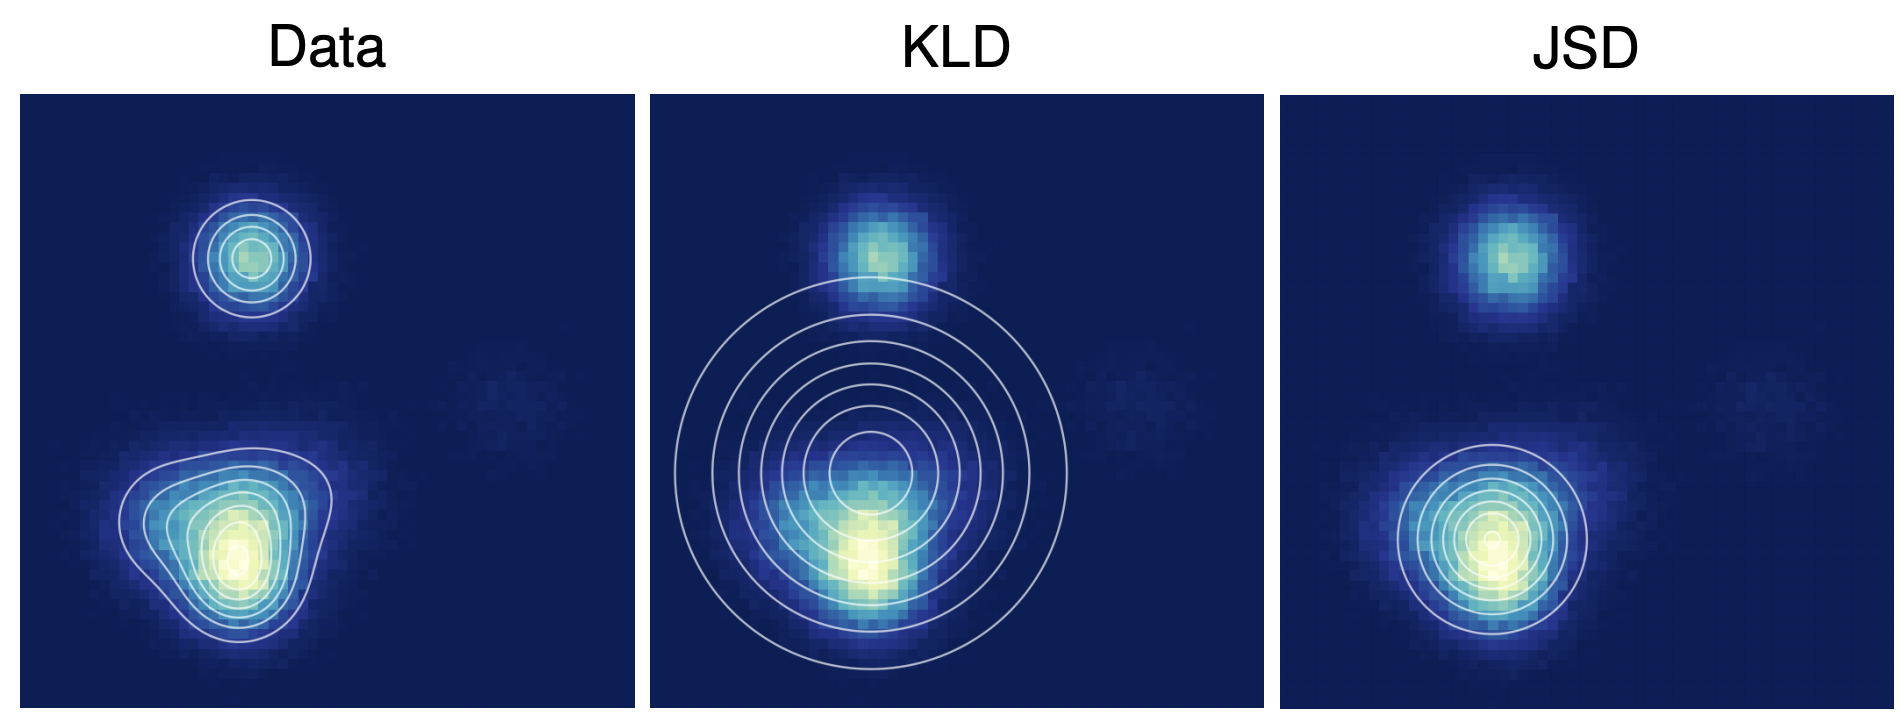
\includegraphics[width=0.75\linewidth]{figs/mode_collapse_1}
	\end{figure}
	\vspace{-0.3cm}
	\begin{figure}
		\centering
		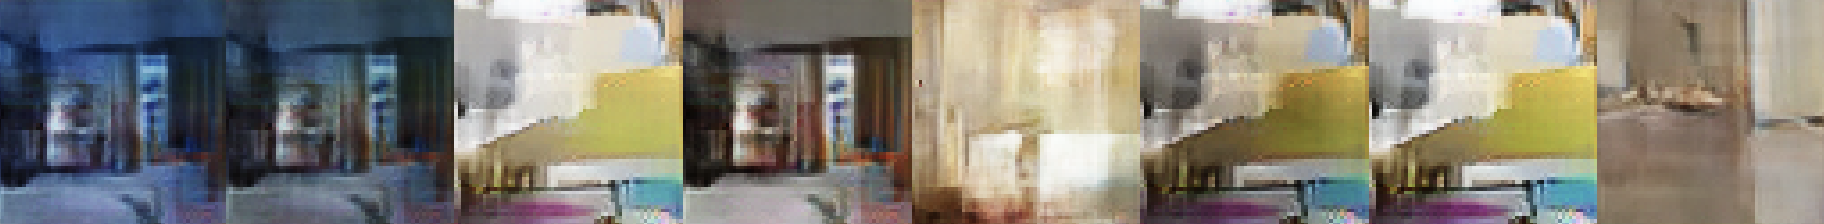
\includegraphics[width=1.0\linewidth]{figs/mode_collapse_4}
	\end{figure}
	\eqpause
	Numerous methods have been proposed to tackle mode collapse: changing architectures, adding regularization terms, injecting noise.
\end{frame}
%=======
\begin{frame}{Jensen-Shannon vs Kullback-Leibler Divergences}
	\begin{itemize}
		\item $\pd(\bx)$ is a fixed mixture of two Gaussians.
		\item $p(\bx | \mu, \sigma) = \cN(\mu, \sigma^2)$.
	\end{itemize}
	\begin{block}{Mode Covering vs. Mode Seeking}
		\vspace{-0.7cm}
		\[
			\KL(\pi \,\|\, p) = \int \pi(\bx) \log \frac{\pi(\bx)}{p(\bx)}d\bx, 
			\quad \KL(p \| \pi) = \int p(\bx) \log \frac{p(\bx)}{\pi(\bx)}d\bx
		\]
		\[
			\JSD(\pi \,\|\, p) = \frac{1}{2} \Bigl[\KL \Bigl(\pi(\bx) \,\|\, \frac{\pi(\bx) + p(\bx)}{2}\Bigr) + \KL \Bigl(p(\bx) \,\|\, \frac{\pi(\bx) + p(\bx)}{2}\Bigr) \Bigr]
		\]
		\vspace{-0.7cm}
		\eqpause
		\begin{minipage}[t]{0.33\columnwidth}
			\begin{figure}
				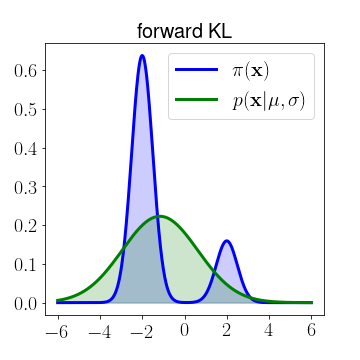
\includegraphics[width=\linewidth]{figs/forward_KL}
			\end{figure}
		\end{minipage}%
		\begin{minipage}[t]{0.33\columnwidth}
			\begin{figure}
				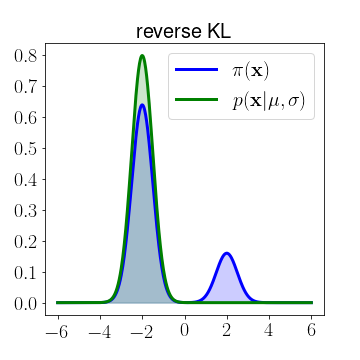
\includegraphics[width=\linewidth]{figs/reverse_KL}
			\end{figure}
		\end{minipage}%
		\begin{minipage}[t]{0.33\columnwidth}
			\begin{figure}
				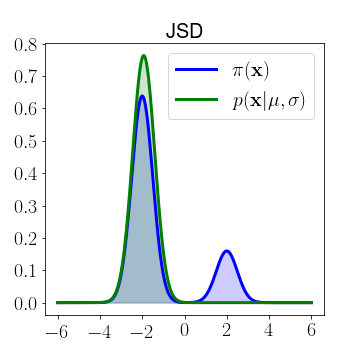
\includegraphics[width=\linewidth]{figs/JSD}
			\end{figure}
		\end{minipage}
		\vspace{-0.3cm}
	\end{block}
\end{frame}
%=======
\section{Wasserstein Distance}
%=======
\begin{frame}{Theoretical Results}
	\myfootnote{\href{https://arxiv.org/abs/1904.08994}{Weng L. From GAN to WGAN, 2019} \\ 
		\href{https://arxiv.org/abs/1701.04862}{Arjovsky M., Bottou L. Towards Principled Methods for Training Generative Adversarial Networks, 2017}}
	\vspace{-0.3cm}
	\begin{itemize}
		\item The dimensionality of $\bz$ is less than that of $\bx$, so $\pt(\bx)$ with $\bx = \bG_{\btheta}(\bz)$ lives on a low-dimensional manifold.
		\eqpause
		\item The true data distribution $\pd(\bx)$ is also supported on a low-dimensional manifold.
		\begin{figure}
			\centering
			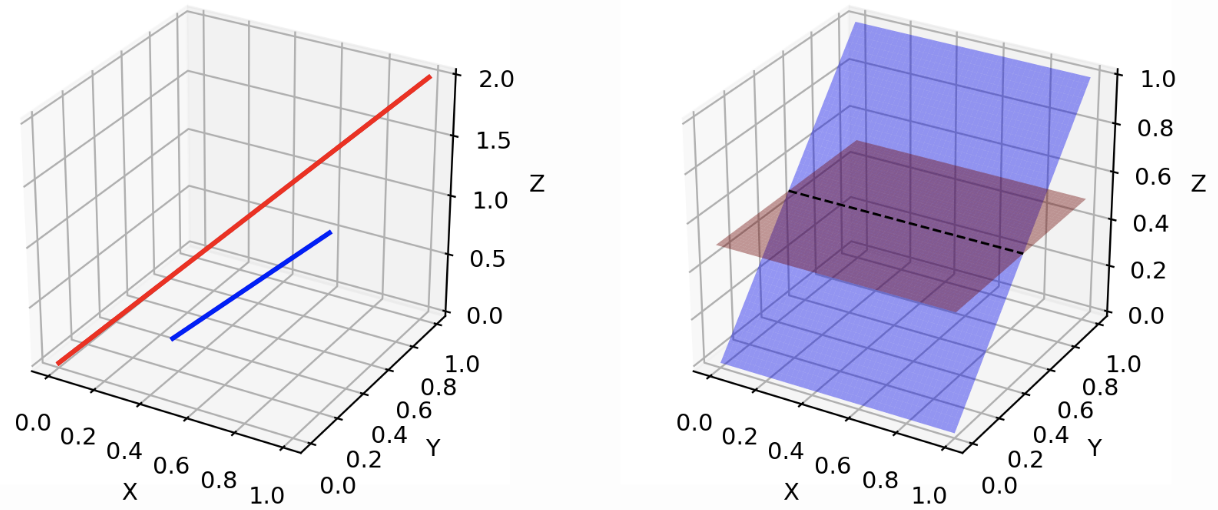
\includegraphics[width=0.55\linewidth]{figs/low_dim_manifold}
		\end{figure}
		\eqpause
		\item If $\pd(\bx)$ and $\pt(\bx)$ are disjoint, a smooth optimal discriminator can exist!
		\eqpause
		\item For such low-dimensional, disjoint manifolds:
		\vspace{-0.2cm}
		\[
			\KL(\pd\,\|\,\pt) = \KL(\pt\,\|\,\pd) = \infty, \quad \JSD(\pd\,\|\,\pt) = \log 2
		\]
	\end{itemize}
\end{frame}
%=======
\begin{frame}{Wasserstein Distance (Discrete)}
	\myfootnotewithlink{https://udlbook.github.io/udlbook/}{Simon J.D. Prince. Understanding Deep Learning, 2023}
	Also known as the \textbf{Earth Mover's Distance}.
	\begin{block}{Optimal Transport Formulation}
		The minimum cost of moving and transforming a pile of "dirt" shaped like one probability distribution to match another.
	\end{block}
	\begin{figure}
		\centering
		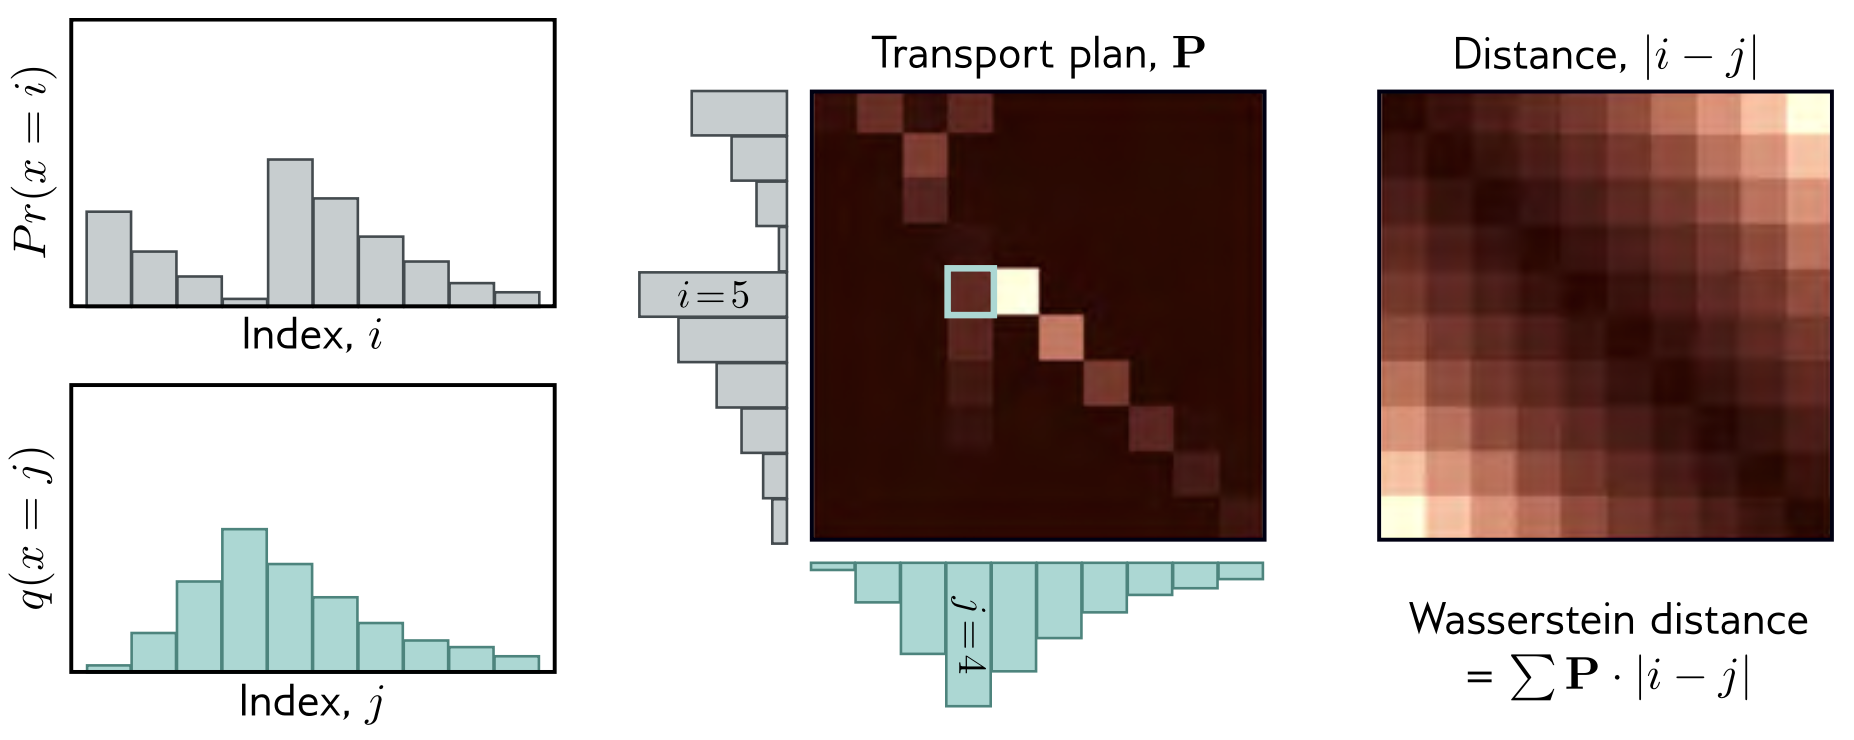
\includegraphics[width=\linewidth]{figs/discrete_wasserstein}
	\end{figure}
\end{frame}
%=======
\begin{frame}{Wasserstein Distance (Continuous)}
	\myfootnotewithlink{https://arxiv.org/abs/1701.07875}{Arjovsky M., Chintala S., Bottou L. Wasserstein GAN, 2017}
	\vspace{-0.5cm}
	{
	\small
	\[
		W(\pi \| p) = \inf_{\gamma \in \Gamma(\pi, p)} \bbE_{(\bx_1, \bx_2) \sim \gamma} \| \bx_1 - \bx_2 \| =  \inf_{{\color{olive}\gamma} \in {\color{teal}\Gamma(\pi, p)}} \int {\color{violet} \| \bx_1 - \bx_2 \|}\, {\color{olive}\gamma (\bx_1, \bx_2)} d \bx_1 d \bx_2
	\]
	}
	\vspace{-0.4cm}
	\begin{itemize}
		\item ${\color{olive}\gamma (\bx_1, \bx_2)}$ is the transport plan: the amount of “dirt” assigned from $\bx_1$ to $\bx_2$.
		\vspace{-0.2cm}
		\[
		\int \gamma(\bx_1, \bx_2) d \bx = p(\bx_2); \quad \int \gamma(\bx_1, \bx_2) d \bx_2 = \pi(\bx_1).
		\]
		\vspace{-0.6cm}
		\item ${\color{teal}\Gamma(\pi, p)}$ denotes the set of all joint distributions $\gamma (\bx_1, \bx_2)$ with marginals $\pi$ and $p$.
		\item ${\color{olive}\gamma(\bx_1, \bx_2)}$ is the mass, ${\color{violet}\|\bx_1 - \bx_2\|}$ is the distance.
	\end{itemize}
	\eqpause
	\begin{block}{Wasserstein Metric}
		\vspace{-0.2cm}
		\[
		W_s(\pi, p) = \inf_{\gamma \in \Gamma(\pi, p)} \Bigl(\bbE_{(\bx_1, \bx_2) \sim \gamma} \|\bx_1 - \bx_2\|^s\Bigr)^{1/s}
		\]
		\vspace{-0.4cm}
	\end{block}
	In our setting, $W(\pi \| p) = W_1(\pi, p)$, which is the transport cost using the $\ell_1$ norm.
\end{frame}
%=======
\begin{frame}{Wasserstein Distance vs KL vs JSD}
	\myfootnote{\href{https://arxiv.org/abs/1904.08994}{Weng L. From GAN to WGAN, 2019} \\ 
		\href{https://arxiv.org/abs/1701.07875}{Arjovsky M., Chintala S., Bottou L. Wasserstein GAN, 2017}}
	\begin{minipage}[t]{0.48\columnwidth}
		Consider two-dimensional distributions:
		\vspace{-0.3cm}
		\[
			\pd(x, y) = (0, U[0, 1])
		\]	
		\[
			p_{\theta}(x, y) = (\theta, U[0, 1])
		\]
	\end{minipage}%
	\begin{minipage}[t]{0.52\columnwidth}
		\vspace{-0.3cm}
		\begin{figure}
			\centering
			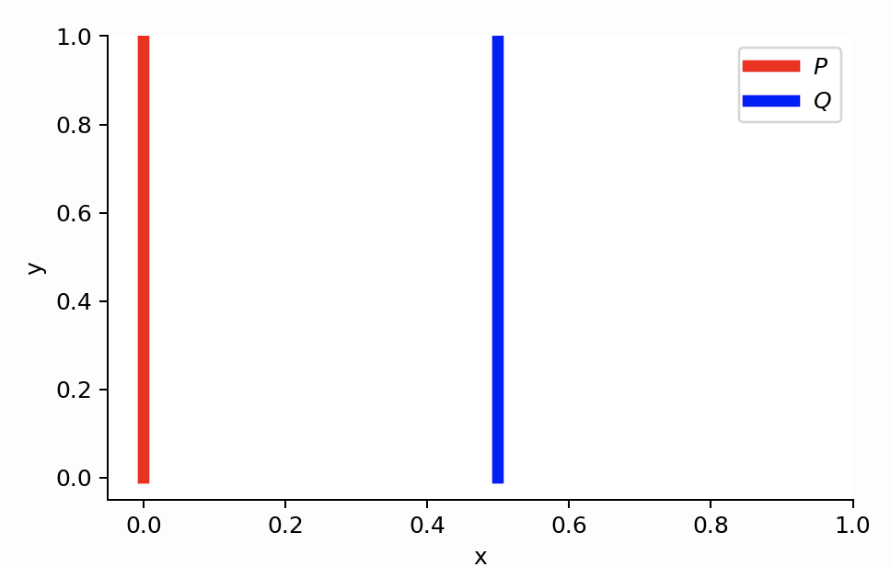
\includegraphics[width=0.8\linewidth]{figs/w_kl_jsd}
		\end{figure}
	\end{minipage}
	\vspace{-0.3cm}
	\eqpause
	\begin{itemize}
		\footnotesize
		\item $\theta = 0$: Both distributions are identical.
		\[
			\KL(\pd \| \pt) = \KL(\pt \| \pd) = \JSD(\pt \| \pd) = W(\pd \| \pt) = 0
		\]
		\vspace{-0.5cm}
		\eqpause
		\item $\theta \neq 0$:
		\vspace{-0.3cm}
		\[
			\KL(\pd \| \pt) = \int_{U[0, 1]} 1 \log \frac{1}{0}\,dy = \infty = \KL(\pt \| \pd)
		\]
		\eqpause
		\[
			\JSD(\pd \| \pt) = \frac{1}{2}\left( \int_{U[0, 1]}1 \log \frac{1}{1/2} dy + \int_{U[0, 1]}1 \log \frac{1}{1/2} dy \right) = \log 2
		\]
		\eqpause
		\[
			W(\pd \| \pt) = |\theta|
		\]
	\end{itemize}
\end{frame}
%=======
\begin{frame}{Wasserstein Distance vs KL vs JSD}
	\myfootnotewithlink{https://arxiv.org/abs/1701.07875}{Arjovsky M., Chintala S., Bottou L. Wasserstein GAN, 2017}
	\begin{block}{Theorem 1}
		Let $\bG_{\btheta}(\bz)$ be (almost) any feedforward neural network, and $p(\bz)$ a prior over $\bz$ such that $\bbE_{p(\bz)} \|\bz\| < \infty$. Then $W(\pd \| \pt)$ is continuous everywhere and differentiable almost everywhere.
	\end{block}
	\eqpause
	\begin{block}{Theorem 2}
		Let $\pi$ be a distribution on a compact space $\cX$ and let $\{p_t\}_{t=1}^\infty$ be a sequence of distributions on $\cX$. 
		\begin{align}
			\KL(\pi \| p_t) &\rightarrow 0 \ \ (\text{or }\KL (p_t\,\|\,\pi) \rightarrow 0) \\
			\JSD(\pi \| p_t) &\rightarrow 0 \\
			W(\pi \| p_t) &\rightarrow 0
		\end{align}
		In summary, as $t \rightarrow \infty$, (1) $\Rightarrow$ (2), and (2) $\Rightarrow$ (3).
	\end{block}
\end{frame}
%=======
\section{Wasserstein GAN}
%=======
\begin{frame}{Wasserstein GAN}
	\myfootnotewithlink{https://arxiv.org/abs/1701.07875}{Arjovsky M., Chintala S., Bottou L. Wasserstein GAN, 2017}
	\begin{block}{Wasserstein Distance}
		\vspace{-0.5cm}
		\small
		\[
		W(\pi \| p) = \inf_{\gamma \in \Gamma(\pi, p)} \bbE_{(\bx_1, \bx_2) \sim \gamma} \| \bx_1 - \bx_2 \| =  \inf_{\gamma \in \Gamma(\pi, p)} \int \|\bx_1 - \bx_2\| \gamma (\bx_1, \bx_2)\, d\bx_1\, d\bx_2
		\]
		\vspace{-0.3cm}
	\end{block}
	\eqpause
	The infimum over all possible $\gamma \in \Gamma(\pi, p)$ is computationally intractable.
	\eqpause
	\begin{block}{Theorem (Kantorovich-Rubinstein Duality)}
		\vspace{-0.3cm}
		\[
			W(\pi \| p) = \frac{1}{K} \max_{\| f \|_L \leq K} \Bigl[ \bbE_{\pi(\bx)} f(\bx)  - \bbE_{p(\bx)} f(\bx)\Bigr]
		\]
		where $f : \bbR^m \rightarrow \bbR$ is $K$-Lipschitz ($\|f\|_L \leq K$):
		\[
			|f(\bx_1) - f(\bx_2)| \leq K \|\bx_1 - \bx_2\|,\quad \forall\ \bx_1, \bx_2 \in \cX.
		\]
		\vspace{-0.6cm}
	\end{block}
	\eqpause
	We can thus estimate $W(\pi \| p)$ using only samples and a function~$f$.
\end{frame}
%=======
\begin{frame}{Wasserstein GAN}
	\myfootnotewithlink{https://arxiv.org/abs/1701.07875}{Arjovsky M., Chintala S., Bottou L. Wasserstein GAN, 2017}
	\begin{block}{Theorem (Kantorovich-Rubinstein Duality)}
		\[
		W(\pd \| \pt) = \frac{1}{K} \max_{\| f \|_L \leq K} \Bigl[ \bbE_{\pd(\bx)} f(\bx)  - \bbE_{\pt(\bx)} f(\bx)\Bigr]
		\]
	\end{block}
	\begin{itemize}
		\item We must ensure that $f$ is $K$-Lipschitz continuous.
		\item Let $f_{\bphi}(\bx)$ be a feedforward neural network parameterized by $\bphi$.
		\item If the weights $\bphi$ are restricted to a compact set $\boldsymbol{\Phi}$, then $f_{\bphi}$ is $K$-Lipschitz.
		\eqpause
		\item Clamp weights within the box $\boldsymbol{\Phi} = [-c, c]^d$ (e.g.\ $c = 0.01$) after each update.
	\end{itemize}
	\begin{multline*}
		K \cdot W(\pd \| \pt) = \max_{\| f \|_L \leq K} \Bigl[ \bbE_{\pd(\bx)} f(\bx)  - \bbE_{\pt(\bx)} f(\bx)\Bigr]\ \geq\ 
		\\  \geq \max_{\bphi \in \boldsymbol{\Phi}} \Bigl[ \bbE_{\pd(\bx)} f_{\bphi}(\bx)  - \bbE_{\pt(\bx)} f_{\bphi}(\bx)\Bigr]
	\end{multline*}
\end{frame}
%=======
\begin{frame}{Wasserstein GAN}
	\myfootnotewithlink{https://arxiv.org/abs/1701.07875}{Arjovsky M., Chintala S., Bottou L. Wasserstein GAN, 2017}
	\begin{block}{Standard GAN Objective}
		\vspace{-0.2cm}
		\[
			\min_{\btheta} \max_{\bphi} \bbE_{\pd(\bx)} \log D_{\bphi}(\bx) + \bbE_{p(\bz)} \log (1 - D_{\bphi}(\bG_{\btheta}(\bz)))
		\]
		\vspace{-0.3cm}
	\end{block}
	\begin{block}{WGAN Objective}
		\vspace{-0.3cm}
		\[
			\min_{\btheta} {\color{violet}W(\pd \| \pt)} \approx \min_{\btheta} {\color{violet}\max_{\bphi \in \boldsymbol{\Phi}} \Bigl[ \bbE_{\pd(\bx)} f_{\bphi}(\bx)  - \bbE_{p(\bz)} f_{\bphi}(\bG_{\btheta}(\bz))\Bigr]}
		\]
		\vspace{-0.3cm}
	\end{block}
	\eqpause
	\begin{itemize}
		\item The discriminator $D$ is replaced by function $f$: in WGAN, it is known as the \textbf{critic}, which is \emph{not} a classifier.
		\item \textit{"Weight clipping is a clearly terrible way to enforce a Lipschitz constraint."}
		\begin{itemize}
			\item If $c$ is large, optimizing the critic is hard.
			\item If $c$ is small, gradients may vanish.
		\end{itemize}
	\end{itemize}	
\end{frame}
%=======
\begin{frame}{Wasserstein GAN}
	\myfootnotewithlink{https://arxiv.org/abs/1701.07875}{Arjovsky M., Chintala S., Bottou L. Wasserstein GAN, 2017}
	\vspace{-0.3cm}
	
	\begin{minipage}[t]{0.6\columnwidth}
		\begin{itemize}
			\item WGAN provides nonzero gradients even if distributions' supports are disjoint.
			\item $\JSD(\pd \| \pt)$ is poorly correlated with sample quality and remains near its maximum value $\log 2 \approx 0.69$.
			\item $W(\pd \| \pt)$ is tightly correlated with quality.
		\end{itemize}
	\end{minipage}%
	\begin{minipage}[t]{0.4\columnwidth}
		\begin{figure}
			\centering
			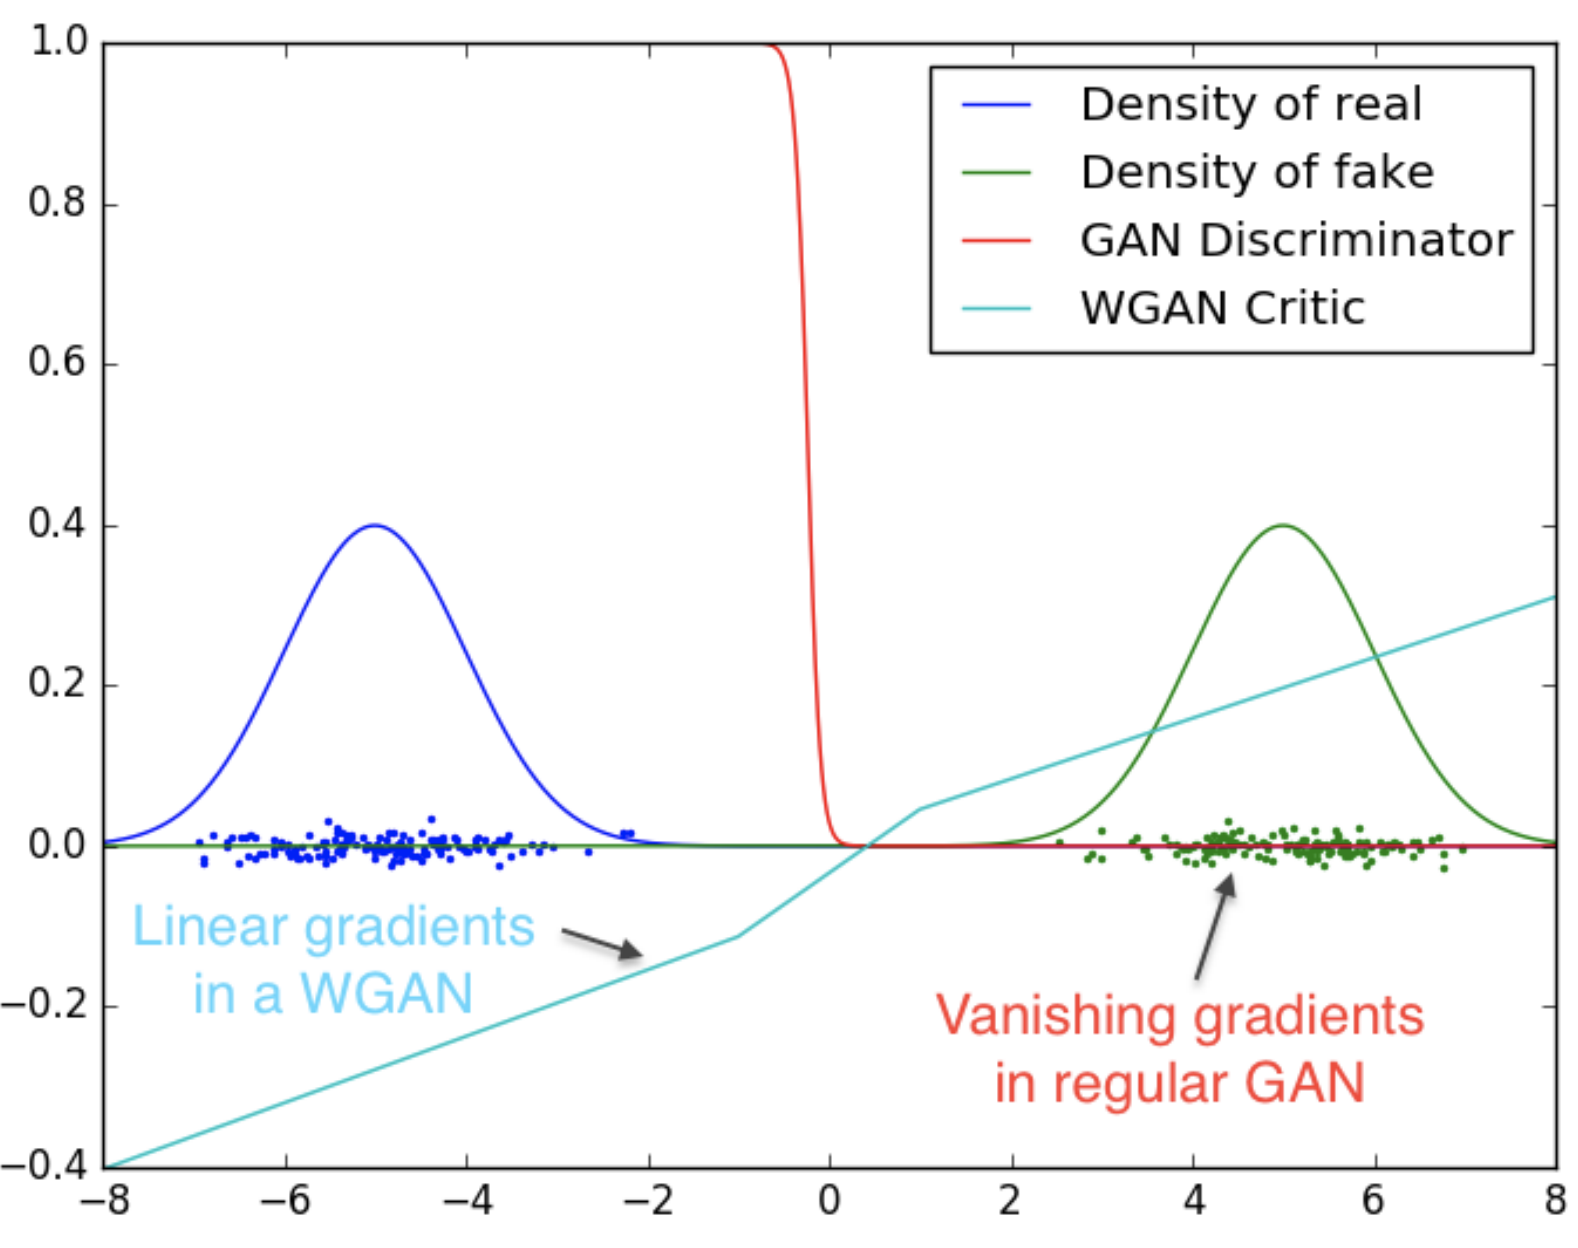
\includegraphics[width=\linewidth]{figs/wgan_toy}
		\end{figure}
	\end{minipage}
	\begin{minipage}[t]{0.5\columnwidth}
		\begin{figure}
			\centering
			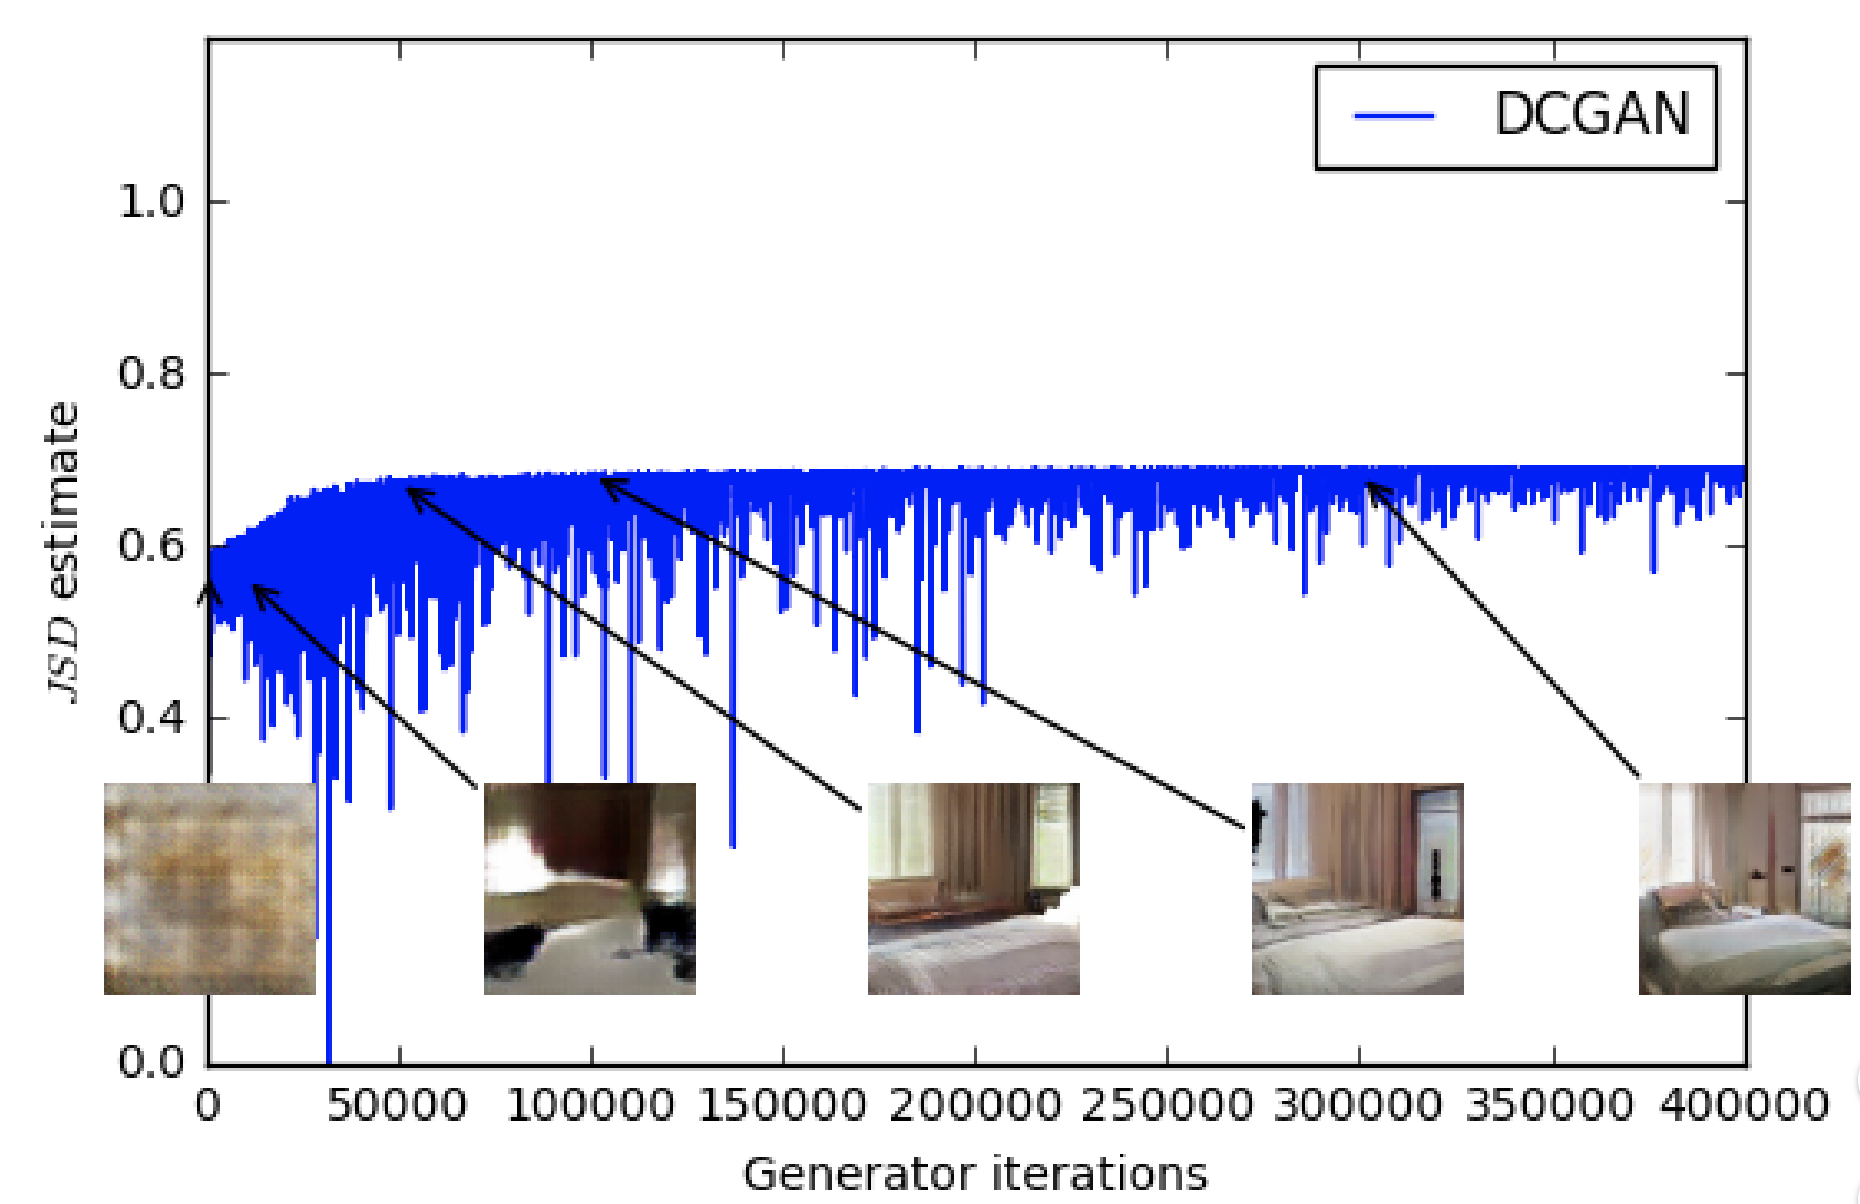
\includegraphics[width=0.95\linewidth]{figs/dcgan_quality}
		\end{figure}
	\end{minipage}%
	\begin{minipage}[t]{0.5\columnwidth}
		\begin{figure}
			\centering
			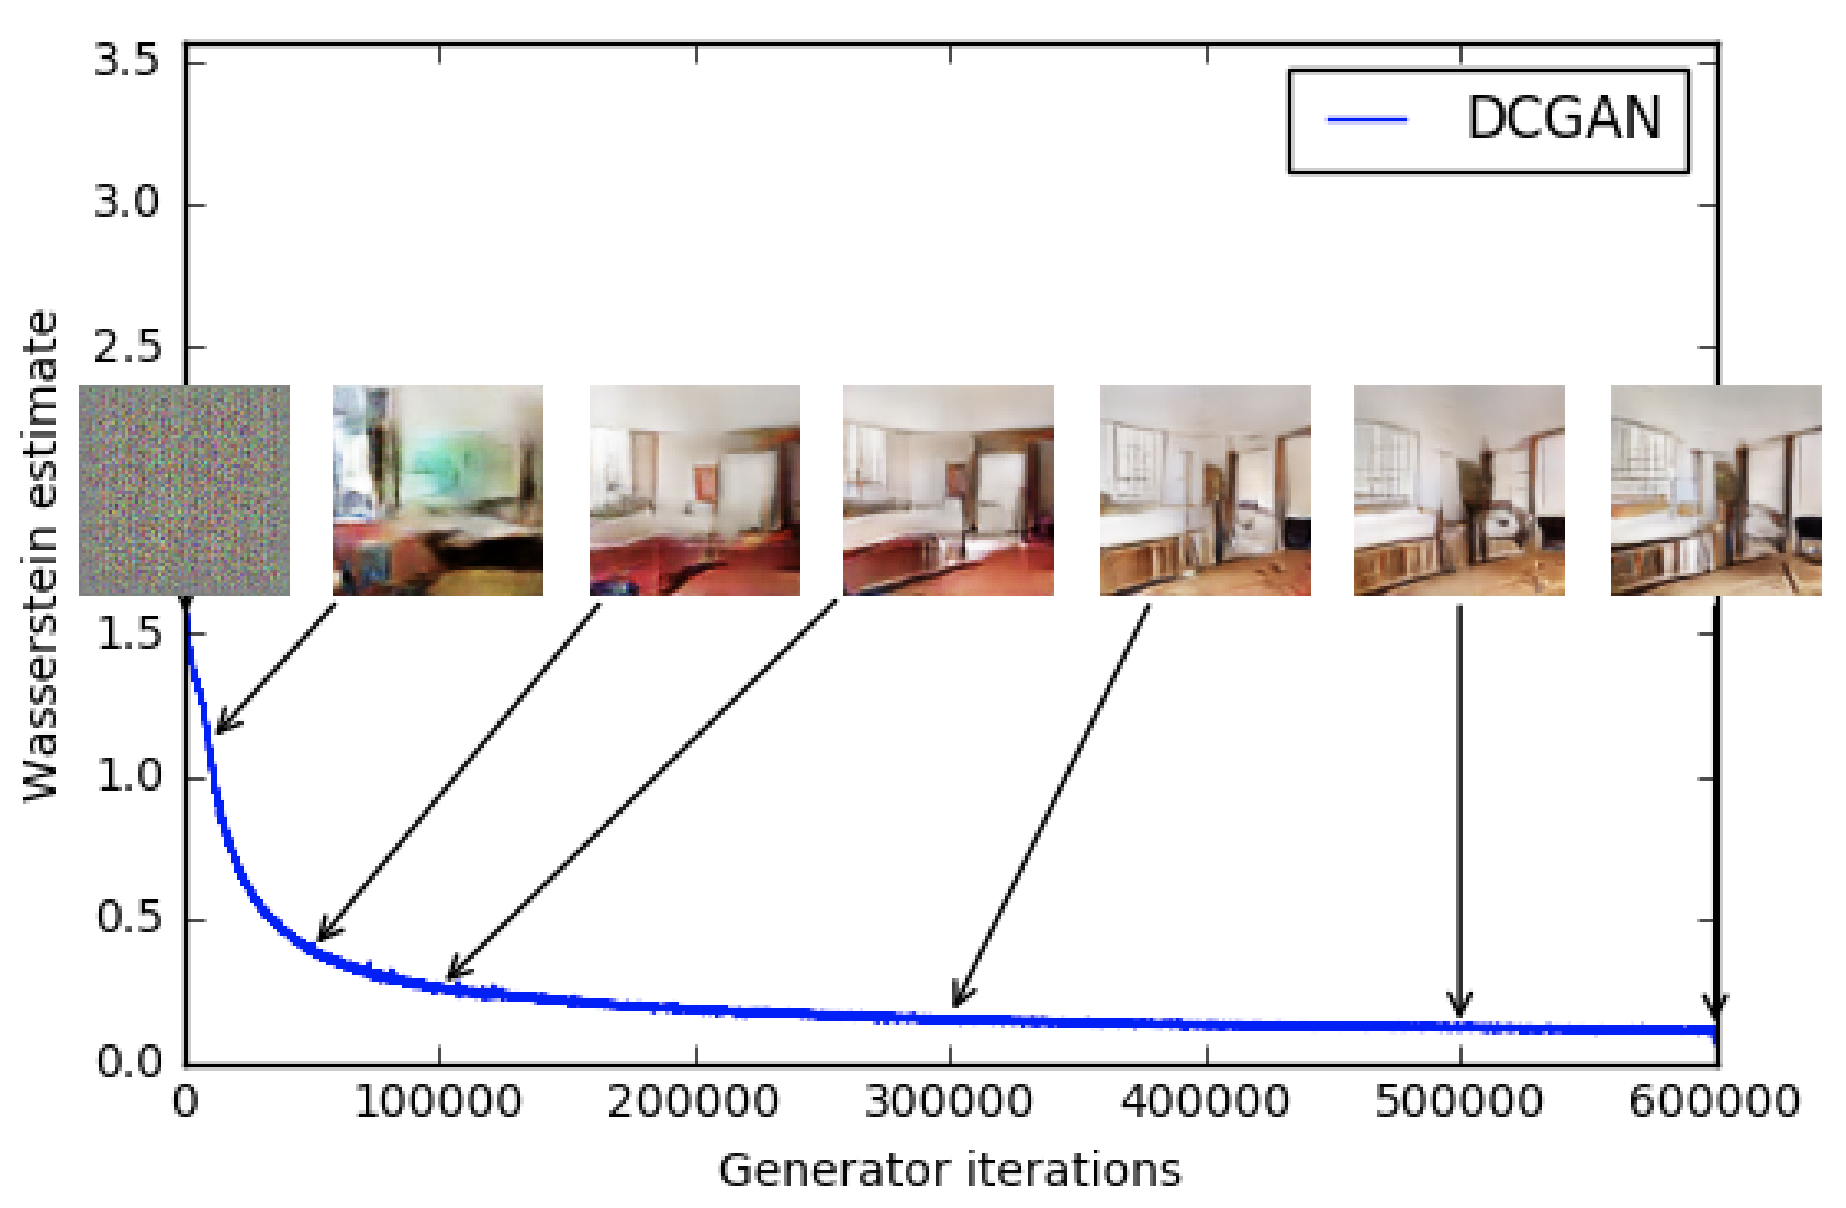
\includegraphics[width=0.95\linewidth]{figs/wgan_quality}
		\end{figure}
	\end{minipage}
\end{frame}
%=======
\begin{frame}{Summary}
	\begin{itemize}
		\item Likelihood is not a reliable metric for generative model evaluation.		
		\vfill
		\item Adversarial learning casts distribution matching as a minimax game.
		\vfill
		\item GANs, in theory, optimize the Jensen-Shannon divergence.
		\vfill
		\item KL and JS divergences fail as objectives when the model and data distributions are disjoint.
		\vfill
		\item The Earth Mover's (Wasserstein) distance provides a more meaningful loss for distribution matching.
		\vfill
		\item Kantorovich-Rubinstein duality allows us to compute the EM distance using only samples.
		\vfill
		\item Wasserstein GAN enforces the Lipschitz condition on the critic through weight clipping---although better alternatives exist.
	\end{itemize}
\end{frame}
%=======
\begin{frame}{Summary}
	\begin{itemize}
		\item
	\end{itemize}
\end{frame}
%=======
\end{document}